\documentclass[11pt,a4paper]{article}
\usepackage[margin=27mm]{geometry}
\usepackage{fontspec,unicode-math,amsmath,booktabs,graphicx,hyperref}
\setmainfont{STIXGeneral}\setmathfont{STIX Two Math}
\setlength{\parindent}{0pt}\setlength{\parskip}{6pt}
\title{Mixes, covers and faithfulness}
\author{Three-original manuscript comparison}\date{}
\begin{document}\maketitle
\textbf{Written papers.} The complete F005, L016 and F007 sources contain 156,570 characters. The entire common theory and all applications contain 103,450 characters. The primary comparison is
\[
\frac{\sum_i c(S_i)}{\sum_j c(U_j)+\sum_i c(A_i)}
=\frac{156570}{34757+68693}
=1.513485.
\]
Here $c$ counts nonwhitespace characters after NFC normalization of complete raw PDF extraction, including page furniture. This primary coordinate was fixed before evaluation and retains the accepted prior Mixes convention. It measures manuscript text, not minimum proof complexity.

All 62 source pages are included. The common papers U, U1 and U2 occupy 5, 4 and 4 pages and contribute 12,615, 11,641 and 10,501 characters. The five application papers occupy 27 pages. Both the F005 exceptional companion and the F007 rank-three companion are paid in full. There is no free old common paper, overlap discount or uncharged cross-topic premise.

\textbf{After acquiring the common theory and required premises.} These conditional factors divide each source by its complete application bundle. They require prior acquisition of all three common papers, both required finite certificates and retained mathematical inputs. Optional validation is not a prerequisite.
\begin{center}\begin{tabular}{llrrr}\toprule
Source & Application bundle & Source & Application & Conditional\\\midrule
F005 & A1+A2 & 57,753 & 31,077 & 1.858384\\
L016 & A3 & 35,506 & 15,125 & 2.347504\\
F007 & A4+A5 & 63,311 & 22,491 & 2.814948\\
\bottomrule\end{tabular}\end{center}
The complete local costs are A1=20,788, A2=10,289, A3=15,125, A4=13,841 and A5=8,650 characters. Full common acquisition is charged once in the whole-topic denominator; it is not charged again inside each conditional factor.

The accepted F005/L016 boundaries retain 35 and 19 dispositions. All three final F005 problems remain unanswered. L016's thin-only lemma needs the stated faithfulness repair; its ancillary smallest-example/Atlas census and further-cover questions are outside principal recovery. This numerical work adds no source, question or formalization credit.
\newpage
\begin{center}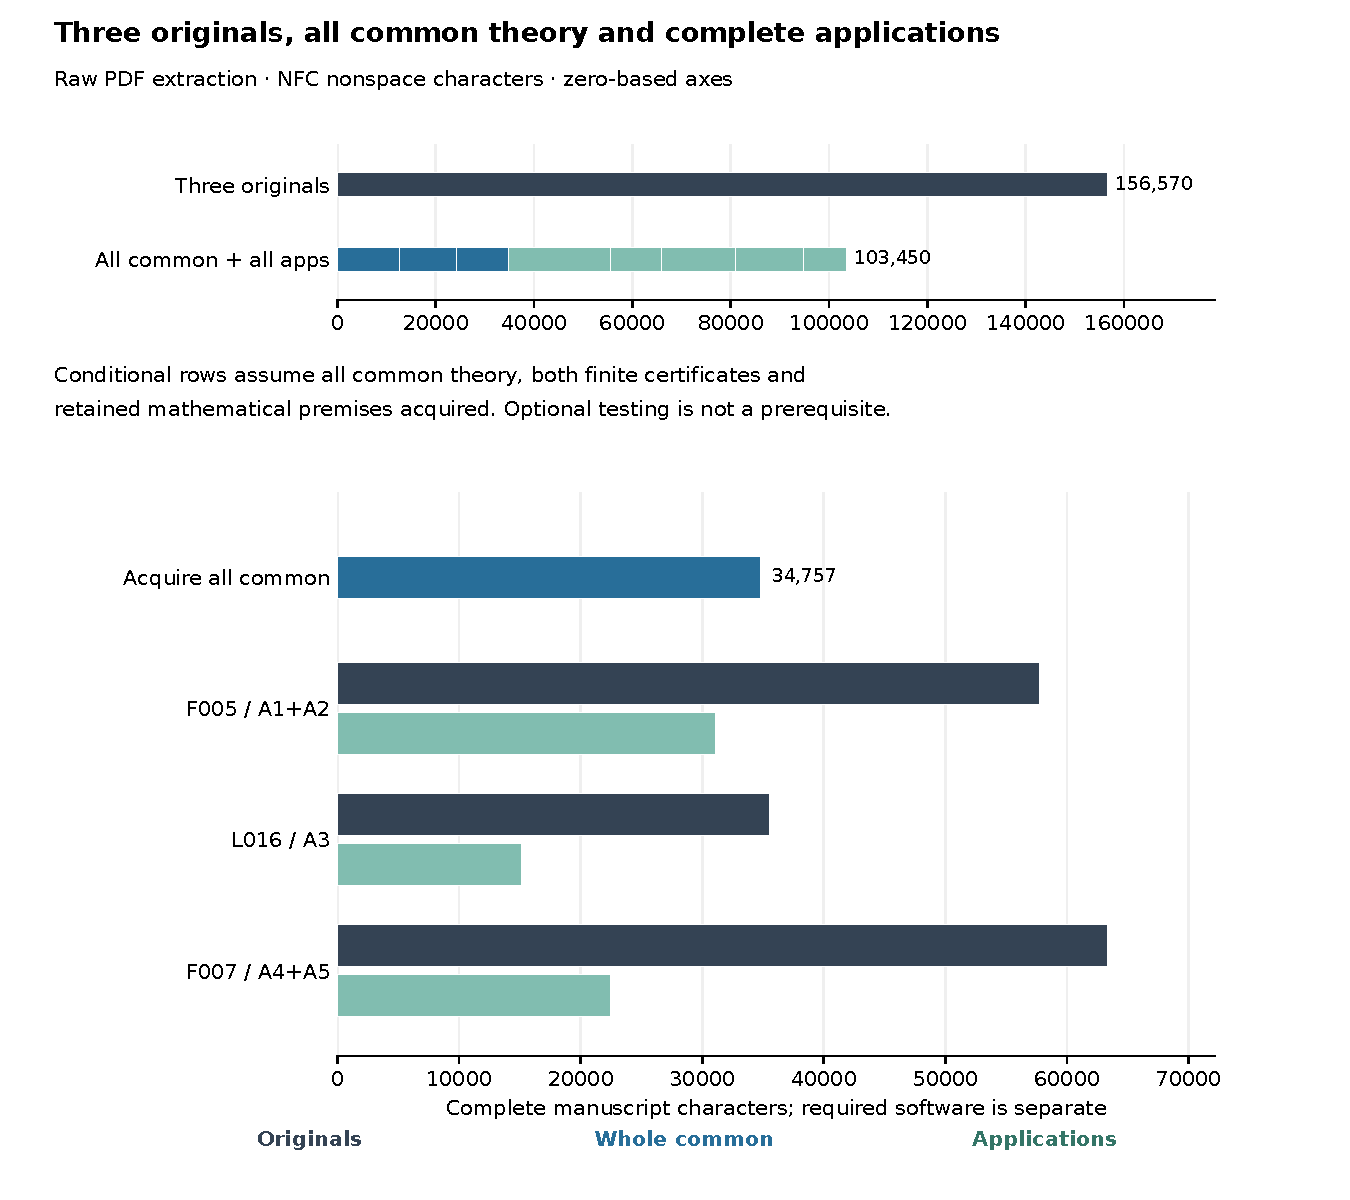
\includegraphics[width=\textwidth]{costs.pdf}\end{center}
The upper graph shows all three common papers and all five application papers as full segments. The lower graph shows the complete common acquisition and all three source/application pairs. Sixteen bars represent manuscript lengths, not ratios or theorem-node counts. Every axis starts at zero. The recorded acquisition order is documentary, with no optimality or sawtooth claim.

\textbf{Symmetric software boundary.} Concrete executable programs are excluded on both sides. Mathematical proofs, algorithm prose, presentations and formulas remain counted. The two finite certificates remain required premises; their exclusion from this manuscript factor does not make them optional. Historical source software is unknown, so no software-inclusive factor is computed.
\newpage
\textbf{Separate whole-file inventory.}
\begin{center}\small\begin{tabular}{lrrr}\toprule
Whole files & Count & NFC nonspace chars & Literal bytes\\\midrule
Required finite certificates & 2 & 2,907 & 3,253\\
Optional validation programs & 6 & 29,862 & 37,745\\
Operational drivers & 6 & 26,552 & 30,936\\
Partial Lean files & 3 & 6,850 & 9,998\\
\bottomrule\end{tabular}\end{center}
The complete required-certificate PDF has 3,431 characters and prints both required programs. F005's certificate also occurs in historical mixed appendix CODE1; this repeated representation is not an additional charge. The retained optional appendix has 7,285 characters and covers only its declared older files; F007's new optional programs have no printed representation here. The historical mixed appendices contain 8,813 and 7,212 characters. Printed and raw representations are never added together. The companion checker has a secondary render role and is counted once among optional files. No mandatory nonprogram data file is hidden in this boundary. Three Lean files contain twelve partial declarations, not a formalization of all source results.

\textbf{Sensitivity of the whole written factor.}
\begin{center}\small\begin{tabular}{lrrr}\toprule
Unit & Raw & Selected & Calibrated\\\midrule
NFC: Whitespace tokens & 1.634193 & 1.617862 & 1.617862\\
NFC: Alphanumeric units & 1.671961 & 1.654123 & 1.652469\\
NFC: Nonspace characters & 1.513485 & 1.494507 & 1.457934\\
NFC: Collapsed-space characters & 1.535114 & 1.516583 & 1.486532\\
NFC: Collapsed UTF-8 bytes & 1.443657 & 1.426755 & 1.439990\\
NFKC: Whitespace tokens & 1.634371 & 1.618040 & 1.618040\\
NFKC: Alphanumeric units & 1.671961 & 1.654123 & 1.652469\\
NFKC: Nonspace characters & 1.517842 & 1.498869 & 1.462302\\
NFKC: Collapsed-space characters & 1.538722 & 1.520196 & 1.490148\\
NFKC: Collapsed UTF-8 bytes & 1.560943 & 1.542698 & 1.519951\\
\bottomrule\end{tabular}\end{center}
All 30 coordinates and 120 exact fractions are retained in JSON/CSV. The 330 prior PDF and 130 prior raw-file cells are unchanged; the 120 new PDF and 40 new raw cells are the independently accepted values. Selected variants remove only exact page furniture; calibration applies the accepted occurrence-bound repairs. F007 has 1,351 substitutions, including decoded Greek-name aliases. Publisher emblems remain in raw text and only their bound footer is removed in selected variants. Full source figures, graphics, retained outside proofs, software/runtime and complete formalization costs remain unknown.

F007's 48 numbered rows and six additional dispositions retain their accepted qualifications. Its unnumbered page-25 chain-class paragraph is not recovered; Problems 1 and 2 remain unanswered. Problem 3 has the natural reconstruction result and the arbitrary-isomorphism result for finite posets with connected full flag graph. No general infinite arbitrary-isomorphism result or historical priority is claimed. The input authorship, distinct review and root adoption are bound; this numerical packet neither reextracts sources nor reruns scientific programs or Lean.
\end{document}
